\documentclass{article}

\usepackage{../preamble/factory, ../preamble/font, ../preamble/math, ../preamble/math_font, ../preamble/style, ../preamble/theorem}

\newtheorem{thr}{Uppgift}

\begin{document}

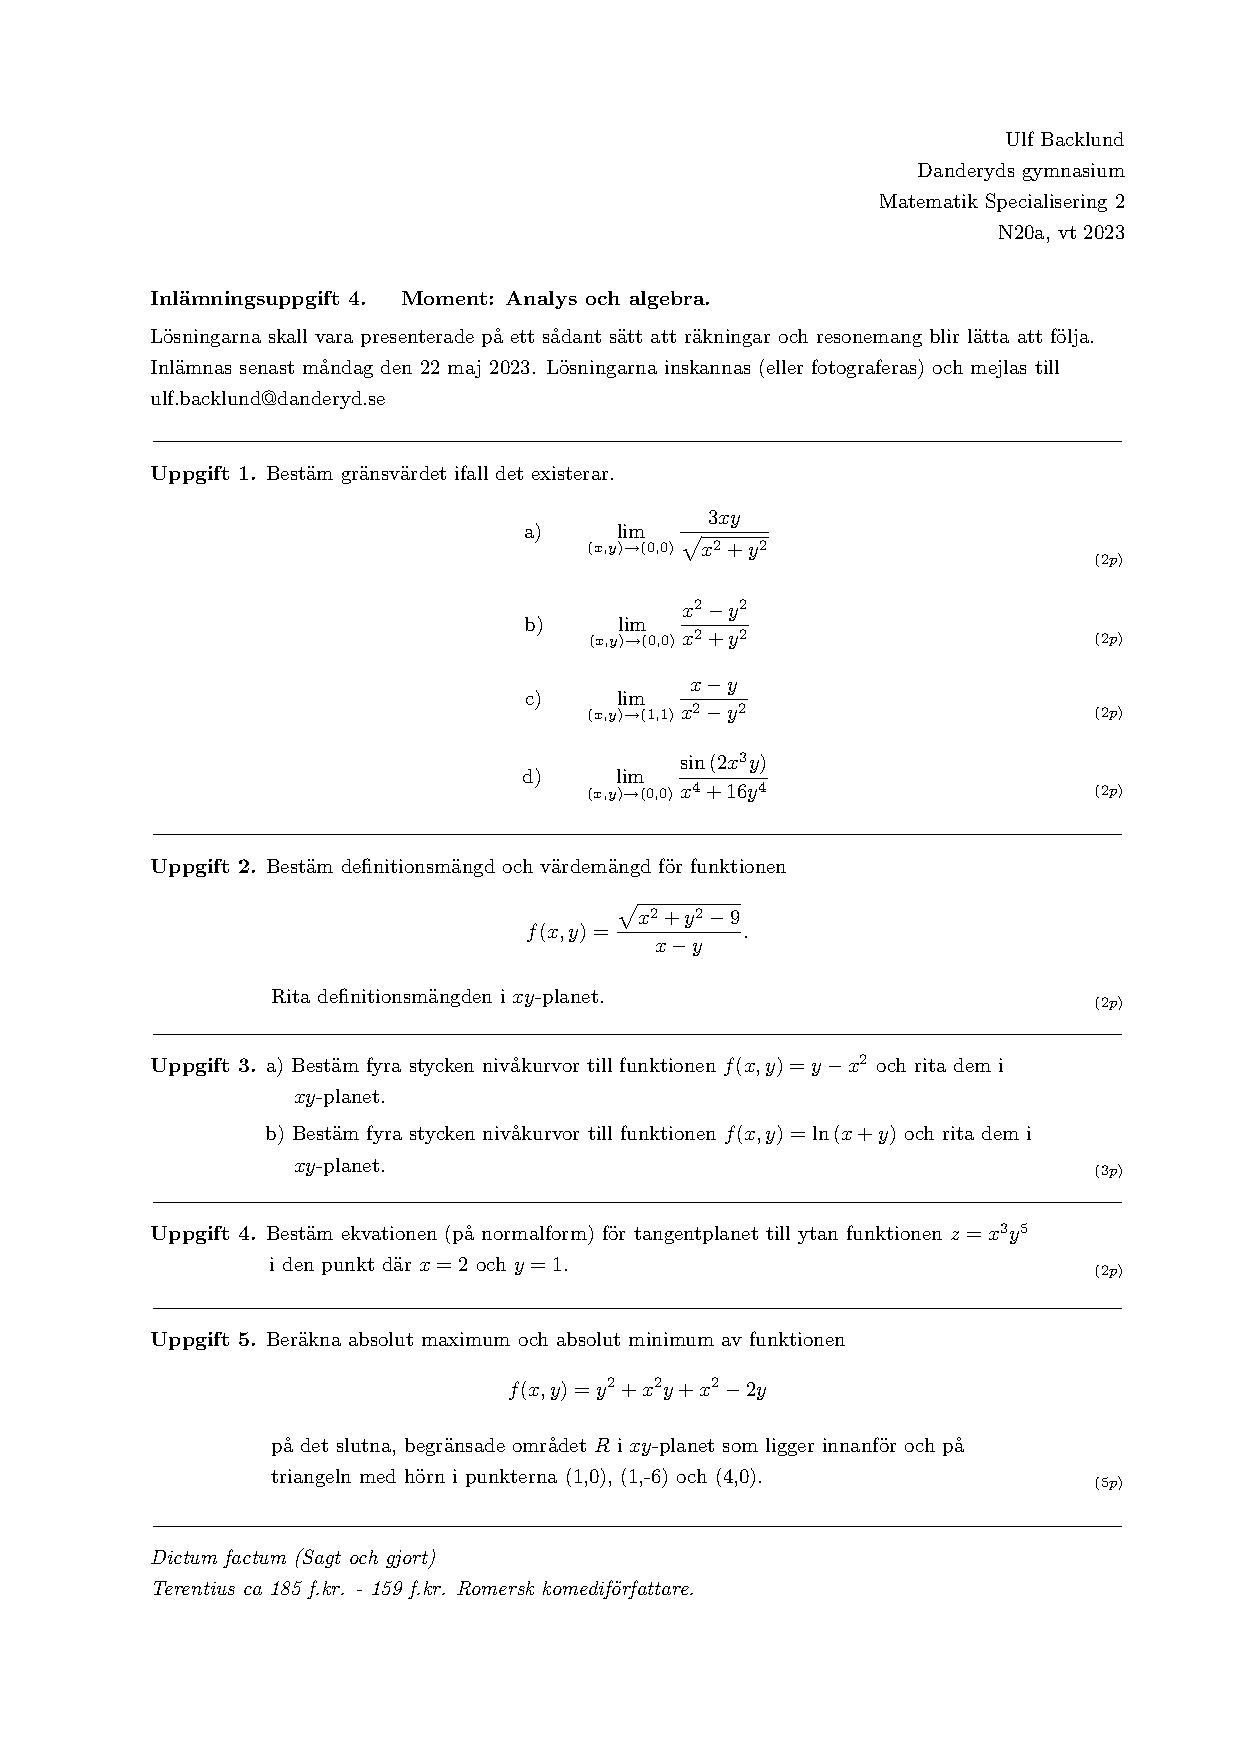
\includepdf{homework_4}

\newpage

\centerline{\large Matematik specialisering 2 inlämning 4}

\vskip 0.1cm

\centerline{\scriptsize Adam Amanbaev}

\vskip 0.5cm

\begin{thr}
\end{thr}

\begin{enumerate}
    \item[a)] Vi undersöker först gränsvärdet längs y-axeln, det vill säga när x=0:

        $$
        \lim_{(x, y)\to(0, 0)}\frac{3xy}{\sqrt{x^2+y^2}}\;
        \underset{(x=0)}\Imp\;
        \lim_{y\to 0}{\frac{3y*0}{\sqrt{y^2+0^2}}}
        =
        \lim_{y\to0}{0}
        =
        0
        $$

        \vskip 0.2cm

        Om gränsvärdet exister ska det alltså vara lika med 0 och detta stämmer redan då $x=0$. Vidare gäller följande för $(x, y)\neq(0, 0)$ och $x\neq0$:

        $$
        0\leq \build f(x, y)-L\build
        =
        \build \frac{3xy}{\sqrt{x^2+y^2}}-0 \build
        =
        \build \frac{3xy}{\sqrt{x^2+y^2}} \build
        \underset{(y^2\geq0)}\leq
        $$

        $$
        \leq\build\frac{3xy}{\sqrt{x^2}}\build
        =
        \build\frac{3xy}{x}\build
        =
        \build3y\build
        $$

        Eftersom |3y| rör sig mot 0 då $(x, y)\to(0, 0)$ ger instängningssatsen följande: 

        $$
        \lim_{(x, y)\to(0, 0)} \frac{3xy}{\sqrt{x^2+y^2}}=0
        $$

        \vskip 0.3cm

    \item[b)] Vi undersöker gränsvärdet längs x-axeln då y=0:
        
        $$
        \lim_{(x, y)\to(0, 0)}{\frac{x^2-y^2}{x^2+y^2}}\;
        \underset{y=0}\Imp\;
        \lim_{x\to0}{\frac{x^2-0}{x^2+0}}
        =
        \lim_{x\to0}{1}
        =
        1
        $$

        \vskip 0.2cm

        Sedan undersöker vi gränsvärdet längs y-axeln då x=0:

        \vskip 0.2cm

        $$
        \lim_{(x, y)\to(0, 0)}{\frac{x^2-y^2}{x^2+y^2}}\;
        \underset{x=0}\Imp\;
        \lim_{y\to0}{\frac{0-y^2}{0+y^2}}
        =
        \lim_{x\to0}{-1}
        =
        -1
        $$

        \vskip 0.2cm

        Eftersom vi har fått två olika värden, 1 och -1, längs två olika kurvor in mot $(0, 0)$ existerar gränsvärdet ej. 

        \vskip 0.3cm
        
    \item[c)] Vi undersöker gränsvärdet längs linjen y=1:

        \vskip 0.1cm

        $$
        \lim_{(x, y)\to(1, 1)}{\frac{x-y}{x^2-y^2}}
        \underset{y=1}\Imp
        \lim_{x\to1}{\frac{x-1}{x^2-1^2}}
        =
        \lim_{x\to1}{\frac{x-1}{(x-1)(x+1)}}
        =
        \lim_{x\to1}{\frac{1}{x+1}}
        =
        \frac{1}{2}
        $$

        \newpage

        Om gränsvärdet existerar är den alltså lika med $\frac{1}{2}$.

        \vskip -0.4cm

        $$
        \lim_{(x, y)\to(1, 1)}{\frac{x-y}{x^2-y^2}}
        =
        \lim_{(x, y)\to(1, 1)}{\frac{x-y}{(x-y)(x+y)}}
        =
        \lim_{(x, y)\to(1, 1)}{\frac{1}{x+y}}
        =
        \lim_{(x, y)\to(1, 1)}{\frac{1}{1+1}}
        =
        \frac{1}{2}
        $$

        \vskip 0.2cm

        Gränsvärdet existerar alltså och är lika med $\frac{1}{2}$.

        \vskip 0.3cm

    \item[d)] Vi undersöker först gränsvärdet längs x-axeln då y=0:

        $$
        \lim_{(x, y)\to(0, 0)}{\frac{\sin(2x^3y)}{x^4+16y^4}}
        \underset{y=0}\Imp
        \lim_{x\to0}{\frac{\sin(0)}{x^4}}
        =
        0
        $$

        Alltså ska gränsvärdet bli lika med 0 om det existerar. Vi undersöker sedan gränsvärdet längs linjen $y=x$:

        \vskip 0.1cm

        $$
        \lim_{(x, y)\to(0, 0)}{\frac{\sin(2x^3y)}{x^4+16y^4}}
        \underset{y=x}\Imp
        \lim_{x\to0}{\frac{\sin(2x^4)}{17x^4}}
        =
        \lim_{x\to0}{\frac{D(\sin(2x^4))}{D(17x^4)}} \;\; \text{\scriptsize(L'Hôpitals regel)}
        $$

        $$
        =
        \lim_{x\to0}{\frac{8x^3\cos(2x^4)}{68x^3}}
        =
        \lim_{x\to0}{\frac{D(8x^3\cos(2x^4))}{D(68x^3)}} \;\; \text{\scriptsize(L'Hôpitals regel)}
        $$

        $$
        =
        \lim_{x\to0}{\frac{24x^2\cos(2x^4)-64x^6\sin(2x^4)}{204x^2}}
        $$

        $$
        =
        \lim_{x\to0}{\frac{D(24x^2\cos(2x^4)-64x^6\sin(2x^4))}{D(204x^2)}} \;\; \text{\scriptsize(L'Hôpitals regel)}
        $$

        $$
        =
        \lim_{x\to0}{\frac{-16x((-3+32x^8)\cos(2x^4)+36x^4\sin(2x^4))}{408x}}
        $$

        $$
        =
        \lim_{x\to0}{\frac{D(-16x((-3+32x^8)\cos(2x^4)+36x^4\sin(2x^4)))}{D(408x)}} \;\; \text{\scriptsize(L'Hôpitals regel)}
        $$

        $$
        =
        \lim_{x\to0}{\frac{16((3-576x^8)\cos(2x^4)+4x^4(-51+64x^8)\sin(2x^4))}{408}}
        $$

        $$
        =
        \lim_{x\to0}{\frac{16((3-576*0^8)\cos(2*0^4)+4*0^4(-51+64*0^8)\sin(2*0^4))}{408}}
        =
        \frac{48}{408}
        $$

        \vskip 0.2cm

        Eftersom vi har fått två olika värden, 0 och $\frac{48}{408}$, längs två olika kurvor in mot $(0, 0)$ existerar gränsvärdet ej.
\end{enumerate}

\newpage

\begin{thr}
\end{thr}

$$
f(x, y)=\frac{\sqrt{x^2+y^2-9}}{x-y}
$$

$$
\therefore\; x-y\neq0 \Och \sqrt{x^2+y^2-9}\geq0
$$

$$
\Imp
y\neq x \Och x^2+y^2-9\geq0
$$

$$
\Imp
y\neq x \Och x^2+y^2\geq9
$$

\vskip 0.2cm

Definitionsmängden är alltså komplementet till mängden av punkter $(x, y)$ sådana att $y=x$ eller $x^2+y^2<9$. Det innebär att definitionsmängden för $f$ är alla punkter som inte ligger på linjen $y=x$ och som inte ligger innanför cirkeln $x^2+y^2=9$.

$$
\therefore D_{f}=\{(x, y)\in \R^2: x^2+y^2\geq9 \Och y\neq x\}
$$

\vskip 0.2cm

Nedan följer en skissering av $f$:s definitionsmängd som är i blått. Det vita är utanför definitionsmängden.

\begin{figure}[h]
    \center
    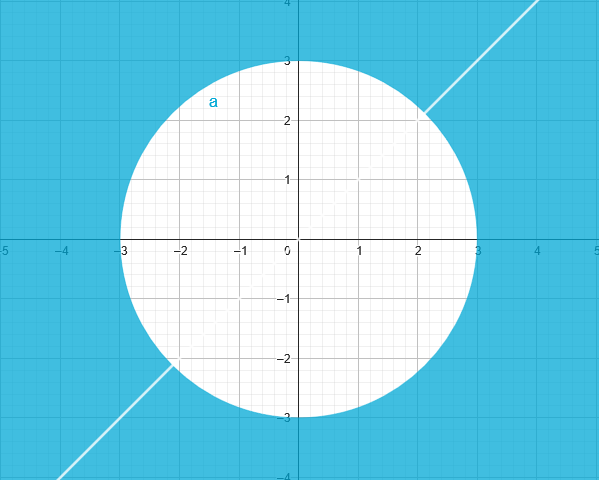
\includegraphics[scale=0.43]{./images/domain}
\end{figure}

Därefter kan vi låta $x=y\pm1$ vilket ger oss följande:

$$
f(x, y)=f(y\pm1, y)=\frac{\sqrt{(y\pm1)^2+y^2-9}}{\pm1}=\pm\sqrt{2y^2\pm2y-8}
$$

Eftersom $g(y)=2y^2\pm2y-8$ oavsett sett tecknet framför $2y$ antar alla reella värden större och lika med 0 antar $\sqrt{g(y)}$ också alla reella värden större och lika med noll. Alltså kan $f$ anta både alla negativa och positiva reella tal samt 0. Värdemängden blir helt enkelt de reella talen.

$$
\therefore\; V_{f}=\{z\in\R\}
$$

\newpage

\begin{thr}
\end{thr}

\begin{enumerate}
    \item[a)] Vi låter $f(x, y)$ vara fyra olika konstanter för att få fyra olika nivåkurvor. Låt dessa vara 0, 1, 2, och 3 för enkelhetens skull:

        $$
        f(x, y)=0=y-x^2 \Imp y=x^2 \;\;  \text{(Röd)}
        $$
        $$
        f(x, y)=1=y-x^2 \Imp y=1+x^2\;\;  \text{(Blå)}
        $$
        $$
        f(x, y)=2=y-x^2 \Imp y=2+x^2\;\;  \text{(Svart)}
        $$
        $$
        f(x, y)=3=y-x^2 \Imp y=3+x^2\;\;  \text{(Grön)}
        $$

        \vskip 0.2cm

        Nedan följer skissering av varje nivåkurva i xy-planet i respektive färg: 

        \vskip 0.5cm

        \begin{figure}[h]
            \center
            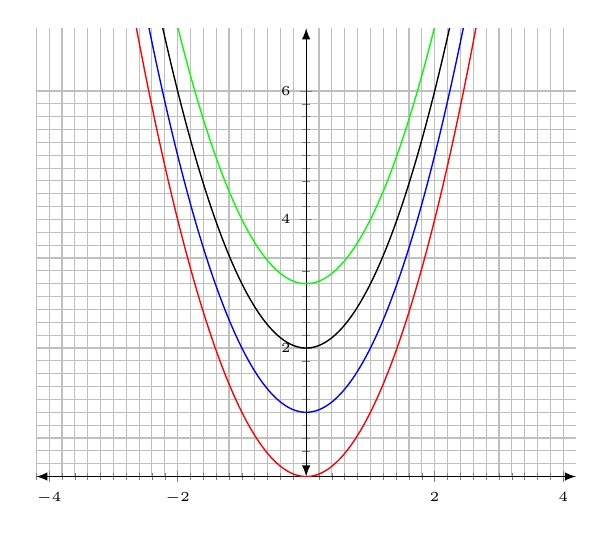
\begin{tikzpicture}
                \begin{axis}[
                    xmin=-2, xmax=2,
                    grid=both,
                    axis lines=middle,
                    minor tick num=9,
                    axis line style={latex-latex},
                    ticklabel style={font=\tiny},
                    axis equal
                    ]
                    \addplot[line width=0.5pt, red, samples=500]{x^2};
                    \addplot[line width=0.5pt, blue, samples=500]{1+x^2};
                    \addplot[line width=0.5pt, black, samples=500]{2+x^2};
                    \addplot[line width=0.5pt, green, samples=500]{3+x^2};
                \end{axis}
            \end{tikzpicture}
        \end{figure}

    \item[b)] För följande nivåkurvor sätter jag $f(x, y)$ till $ln(1), ln(2), ln(3)$ och $ln(4)$:

        $$
        f(x, y)=ln(1)=ln(x+y) \Imp e^{ln(1)}=e^{ln(x+y)} \Imp y=1-x \;\; \text{(Röd)}
        $$
        $$
        f(x, y)=ln(2)=ln(x+y) \Imp e^{ln(2)}=e^{ln(x+y)} \Imp y=2-x \;\; \text{(Blå)}
        $$
        $$
        f(x, y)=ln(3)=ln(x+y) \Imp e^{ln(3)}=e^{ln(x+y)} \Imp y=3-x \;\; \text{(Svart)}
        $$
        $$
        f(x, y)=ln(4)=ln(x+y) \Imp e^{ln(4)}=e^{ln(x+y)} \Imp y=4-x \;\; \text{(Grön)}
        $$

        \vskip 0.3cm

        Nedan följer skissering av varje nivåkurva i xy-planet i respektive färg:

        \newpage

        \begin{figure}[h]
            \center
            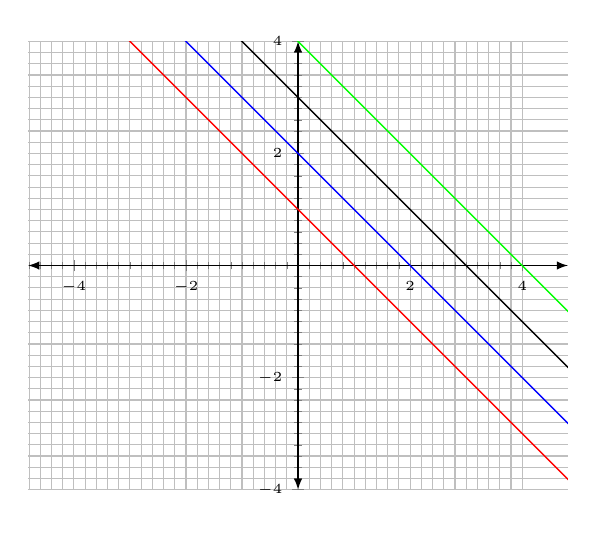
\begin{tikzpicture}
                \begin{axis}[
                    xmin=-4, xmax=4,
                    ymin=-4, ymax=4, 
                    grid=both,
                    axis lines=middle,
                    minor tick num=9,
                    axis line style={latex-latex},
                    ticklabel style={font=\tiny},
                    axis equal
                    ]
                    \addplot[line width=0.5pt, red, samples=200]{1-x};
                    \addplot[line width=0.5pt, blue, samples=200]{2-x};
                    \addplot[line width=0.5pt, black, samples=200]{3-x};
                    \addplot[line width=0.5pt, green, samples=200]{4-x};
                \end{axis}
            \end{tikzpicture}
        \end{figure}
\end{enumerate}

\newpage

\begin{thr}
\end{thr}
%(2, 1)

Vi ska bestämma tangentplanet till $z=x^3y^5$ i punkten $(2, 1, 2^3*1^5)$:

$$
z=f(x, y)=x^3y^5
$$

$$
\therefore\; f_{x}=3x^2y^5 \Och f_{y}=5y^4x^3
$$

$$
\Imp\;
f_{x}(2, 1)=3*2^2*1^5=12 
\Och
f_{y}(2, 1)=5*1^4*2^3=40
$$

\vskip 0.2cm

Tangentplanets ekvation vid punkten $(2, 1, 8)$ på normalform blir därmed:

\vskip 0.2cm

$$
\mathbf{E}:\; f_{x}(2, 1)(x-2)+f_{y}(2, 1)(y-1)-(z-f(2, 1))=0
$$

$$
\Imp
\mathbf{E}:\; 12(x-2)+40(y-1)-(z-8)=0
$$

$$
\Imp
\mathbf{E}:\; 12x+40y-z=56
$$

\newpage

\begin{thr}
\end{thr}

\begin{figure}[h]
    \center
    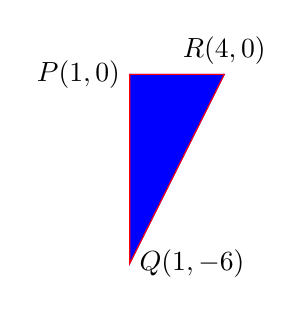
\begin{tikzpicture}
        \coordinate[label=left:{$P(1,0)$}](p) at (4mm,0mm);
        \coordinate[label=right:{$Q(1,-6)$}](q) at (4mm,-24mm);
        \coordinate[label=above:{$R(4,0)$}] (r) at (16mm,0mm);

        \draw[fill, blue] (p) -- (q) -- (r) -- cycle;
        \draw[red] (p) -- (q) -- (r) -- cycle;
    \end{tikzpicture}
\end{figure}

Låt det blåa området betecknas av $D$ där den röda randen inte inkluderas. Vi börjar med att söka alla punkter inom $D$ som eventuellt kan ge ett absolut minimum eller maximum genom att lösa ekvationssystemet där partialderivatorna till $f(x, y)=y^2+x^2y+x^2-2y\;$ är noll ty horisontellt tangentplan:

$$
\begin{cases}
    f_{x}=0 \\
    f_{y}=0 
\end{cases}
\Imp
\begin{cases}
    2xy+2x=0 \\
    2y+x^2-2=0
\end{cases}
\Imp
\begin{cases}
    2x(y+1)=0 \\
    2y+x^2-2=0
\end{cases}
$$

\vskip 0.2cm

Ekvationen $2x(y+1)=0$ ger två fall; $x=0$ och $y=-1$. Insättning av dess i andra ekvationen ger:

$$
\begin{cases}
    x=0 \\
    2y+0^2-2=0
\end{cases}
\Imp
\begin{cases}
    x=0 \\
    y=1
\end{cases}
$$

\vskip 0.2cm

$$
\begin{cases}
    y=-1 \\
    -2+x^2-2=0
\end{cases}
\Imp
\begin{cases}
    y=-1 \\
    x^2=4
\end{cases}
\Imp
\begin{cases}
    y=-1 \\
    x=\pm2
\end{cases}
$$

\vskip 0.2cm

Den enda av dessa lösningar som ligger inom $D$ är $(2, -1)$. Vidare ska vi studera randen, det röda i bilden ovan, som kan delas in i tre delar; linjen som går mellan $P$ och $Q$, linjen som går mellan $P$ och $R$ och linjen som går mellan $Q$ och $R$:

\vskip 0.3cm

\begin{enumerate}
    \item[]
        På linjen mellan $P$ och $Q$ gäller $x=1$ vilket ger:

        $$
        f(1, y)=g(y)=y^2+y-2y+1, \; -6\leq y\leq0
        $$

        \vskip 0.2cm

        $g(y)$ är strikt minskande då $-6\leq y\leq0$ ty $g^{'}(y)=2y-1$ vilket ger oss två punkter; ett potentiellt minimum vid $(1, 0)$ och ett potentiell maximum vid $(1, -6)$. 

        \vskip 0.3cm

        På linjen mellan $P$ och $R$ gäller $y=0$ vilket ger:

        $$
        f(x, 0)=g(x)=x^2, \; 1\leq x\leq4
        $$

        \newpage

        $g(x)$ är strikt ökande då $1\leq x\leq4$ ty $g^{'}(x)=2x$ vilket ger oss två punkter; ett potentiellt minimum vid $(1, 0)$ och ett potentiellt maximum vid $(4, 0)$.

        \vskip 0.3cm

        På linjen mellan $Q$ och $R$ gäller $y=2x-8$ vilket ger:

        $$
        f(x, 2x-8)=h(x)=(2x-8)^2+x^2(2x-8)+x^2-2(2x-8)
        $$
        $$
        =
        2x^3-3x^2-36x+80,\; 1\leq x\leq4
        $$

        $$
        \therefore\;
        h^{'}(x)=6x^2-6x-36=0
        \Imp
        x_{1}=-2 \Och x_{2}=3
        \underset{1\leq x\leq4}\Imp
        x=3
        $$

        \vskip 0.2cm

        $h(x)$ har alltså en extrempunkt då $x=3$ som ger punkten $(3, -2)$ att pröva och vi behöver även pröva ändpunkterna vid $(1, -6)$ och $(4, 0)$. Detta ger oss alltså tre punkter.
\end{enumerate}

Sammantaget behöver vi pröva punkterna $(2, -1)$, $(1, 0)$, $(1, -6)$, $(4, 0)$ och $(3, -2)$:

$$
f(2, -1)=(-1)^2+2^2*(-1)+2^2-2*(-1)=3
$$
$$
f(1, 0)=0^2+1^2*0+1^2-2*0=1
$$
$$
f(1, -6)=(-6)^2+1^2*(-6)+1^2-2*(-6)=43
$$
$$
f(4, 0)=0^2+4^2*0+4^2-2*0=16
$$
$$
f(3, -2)=(-2)^2+3^2*(-2)+3^2-2*(-2)=-1
$$

\vskip 0.2cm

Funktionen $f$ har alltså det absoluta minimumet -1 som antas vid $(3, -2)$ och det absoluta maximumet 43 som antas vid $(1, -6)$ inom det givna området.

\end{document}
